\begin{minipage}[l]{0.5\textwidth}
 \begin{exerciseS}[Giochi d'acqua]
  In un gioco d'acqua ($\rho=999\ kg/m^3$), un disco di diametro $D=35\ cm$ viene sollevato 
  da un getto che fuoriesce con velocit\`{a} $V_0=10\ m/s$ da un foro di diametro $d_0=8\ cm$ concentrico 
  all'asse del disco, cos\`i come illustrato schematicamente in figura. Noto che in condizioni 
  stazionarie la quota raggiunta dal disco \`{e} di poco superiore alla quota $H=2\ m$, si richiede 
  di determinare:
  \begin{itemize}
   \item[1.1)] la velocità $V_1$ e il diametro $d_1$ del getto alla quota $H$
         supponendo trascurabili tra le sezioni $0$ e $1$ sia la curvatura delle linee di flusso 
         che ogni forma di dissipazione;
   \item[1.2)] lo spessore $h$ del film d'acqua all'estremit\`{a} del disco assumendo
         che il profilo di velocit\`{a} radiale sia lineare con velocit\`{a} massima $V_2=V_1$.     
   \item[1.3)] la massa $m$ del disco considerando trascurabili sia gli sforzi viscosi all'interfaccia tra l'atmosfera 
               circostante ($P_{atm}=101325\ Pa$) e il getto d'acqua che la forza gravitazionale agente sul fluido 
               tra la quota $H$ e la quota del disco.
  \end{itemize}
 \end{exerciseS}
 \textit{Per la risoluzione del problema si assumano condizioni di assialsimmetria.}
\end{minipage}
\hspace{3mm}
\begin{minipage}[r]{0.5\textwidth}
 \centering
  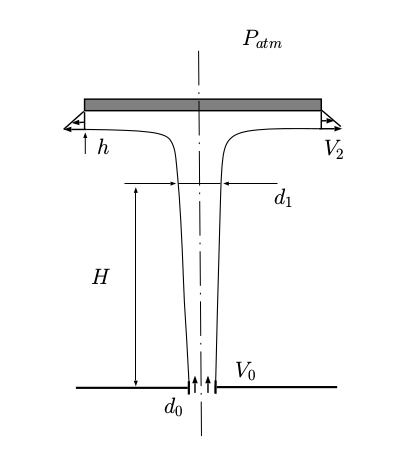
\includegraphics[width=1.0\textwidth]{./fig/jet}
\end{minipage}

\sol

\partone
 Teorema di Bernoulli nell'ipotesi di stazionarietà, fluido incomprimibile, non viscoso, irrotazionale. Bilanci integrali.
 
\parttwo
\begin{itemize}

\item Il primo punto viene risolto mettendo a sistema il teorema di Bernoulli e la 
continuità.
\begin{equation}
\begin{cases}
  \frac{1}{2} \rho V_0^2  = \frac{1}{2}\rho V_1^2(z) + \rho g H\\
  V_0 d_0^2 = V_1 d_1^2
\end{cases} \qquad \Rightarrow \qquad 
\begin{cases}
  V_1 = V_0\sqrt{1 - 2 g H / V_0^2} \\
  d_1 = \displaystyle\left[1 - \frac{2 g H}{V_0^2}\right]^{-\frac{1}{4}} d_0
\end{cases}
\end{equation}

\item Il secondo punto viene risolto utilizzando solamente il bilancio di massa.
\begin{equation}
  Q = \frac{\pi}{4} \rho V_0 d_0^2 = \frac{\pi}{4} \rho V_1 d_1^2 = \frac{\pi}{2} D h V_2 \qquad \Rightarrow \qquad h = \frac{d_1^2}{2 D}
\end{equation}

\item Il terzo punto viene risolto applicando il bilancio della quantità di moto in
direzione verticale per trovare la forza applicata dal disco al fluido. Infine si 
scrive l'equilibrio del disco soggetto alla stessa forza con verso opposto (principio
di azione e reazione) e al proprio peso.

Dal bilancio si ottiene che la componente verticale della forza che si scambiano fluido e disco è uguale a $\rho V_1^2 \frac{\pi}{4} d_1^2$. La massa del disco è quindi $m = \frac{\pi}{4} d_1^2 \frac{\rho V_1^2}{g}$

\end{itemize}





